\documentclass[11pt]{article}

\usepackage[margin=1in]{geometry}
\usepackage{amsmath, amssymb, amsthm}
\usepackage{mathtools}
\usepackage{enumitem}
\usepackage{hyperref}
\usepackage{graphicx}
\usepackage{tikz}
\usetikzlibrary{arrows.meta, positioning, calc,fit}

\title{Simulation Plan}
\author{Oren Ram \\ Ziv Abraham}
\date{\today}

\begin{document}
\maketitle

\begin{figure}[htbp]
    \centering
\resizebox{\textwidth}{!}{%
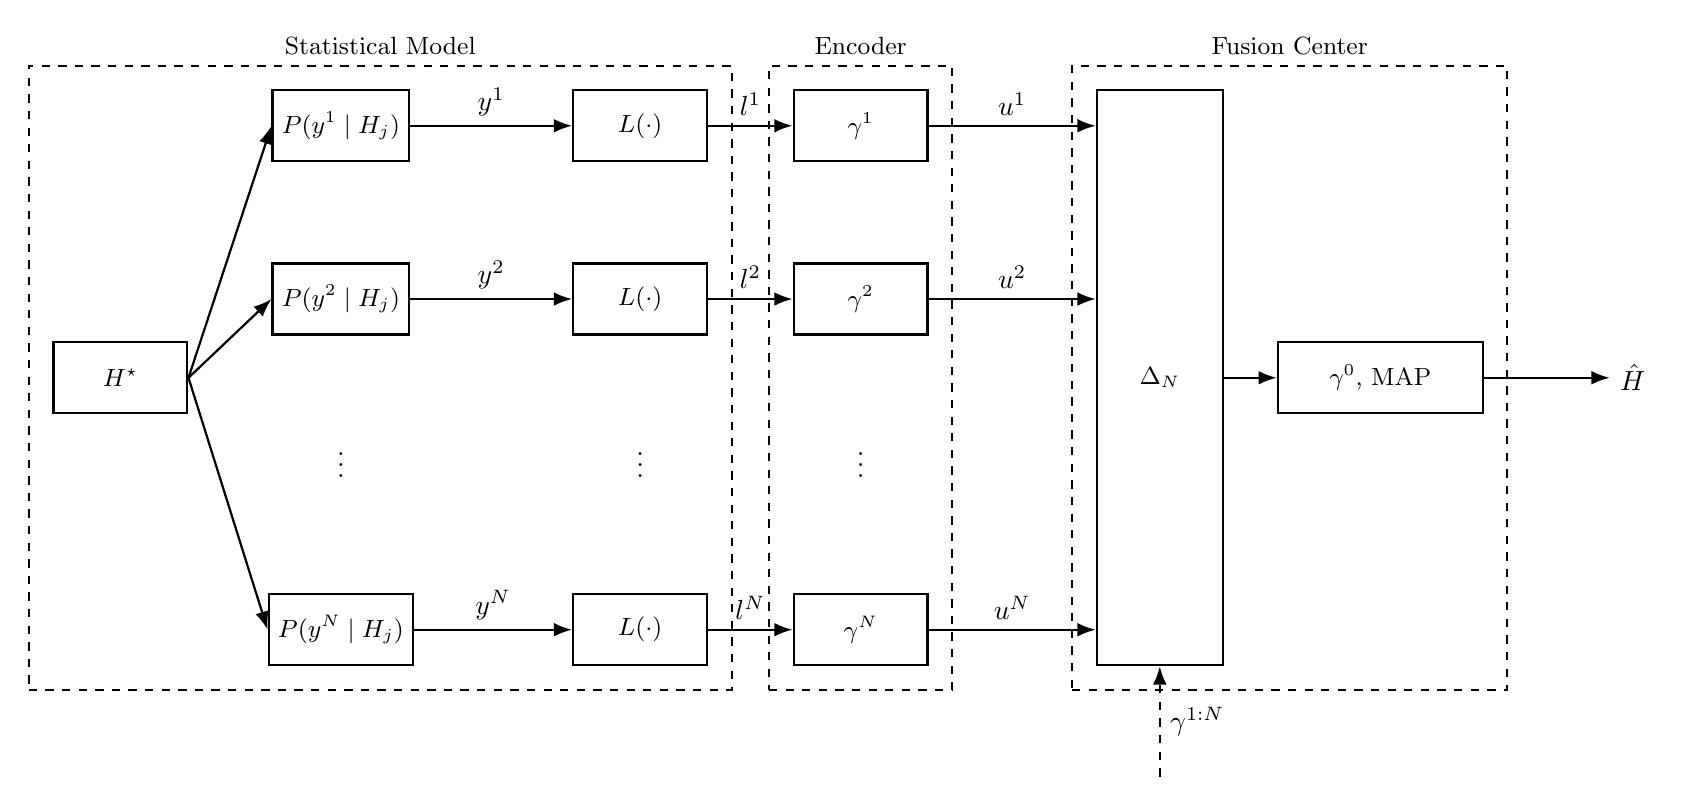
\begin{tikzpicture}[
        box/.style={draw, minimum width=1.7cm, minimum height=0.9cm, align=center, font=\small},
        bigbox/.style={draw, align=center, font=\small},
        ->, >=Latex, thick
    ]
% Source of the hypothesis
\node[box] (H) at (0,0) {$H^\star$};

% Sensor branch i = 1
\node[box] (S1) at (2.8,3.2)  {$P(y^1 \mid H_j)$};
\node[box] (L1) at (6.6,3.2)  {$L(\cdot)$};
\node[box] (E1) at (9.4,3.2)  {$\gamma^1$};

% Sensor branch i = 2
\node[box] (S2) at (2.8,1.0)  {$P(y^2 \mid H_j)$};
\node[box] (L2) at (6.6,1.0)  {$L(\cdot)$};
\node[box] (E2) at (9.4,1.0)  {$\gamma^2$};

% Continuation
\node at (2.8,-1.0) {$\vdots$};
\node at (6.6,-1.0) {$\vdots$};
\node at (9.4,-1.0) {$\vdots$};

% Sensor branch i = N
\node[box] (SN) at (2.8,-3.2) {$P(y^N \mid H_j)$};
\node[box] (LN) at (6.6,-3.2) {$L(\cdot)$};
\node[box] (EN) at (9.4,-3.2) {$\gamma^N$};

% Fusion block, spans the height of all branches
\node[bigbox, minimum width=1.6cm, minimum height=7.3cm] (D) at (13.2,0) {$\Delta_N$};

% Decision block
\node[box, minimum width=2.6cm] (G0) at (16.0,0) {$\gamma^0$, MAP};

% Statistical model enclosure
\node[draw, dashed, thick, inner sep=0.3cm, fit=(H)(S1)(SN)(L1)(LN),
      label={[font=\small]above:Statistical Model}] (SMbox) {};

% Encoder enclosure
\node[draw, dashed, thick, inner sep=0.3cm, fit=(E1)(EN),
      label={[font=\small]above:Encoder}] (ENCbox) {};

% Fusion center enclosure
\node[draw, dashed, thick, inner sep=0.3cm, fit=(D)(G0),
      label={[font=\small]above:Fusion Center}] (FCbox) {};

% Source to each sensor
\draw (H.east) -- (S1.west);
\draw (H.east) -- (S2.west);
\draw (H.east) -- (SN.west);

% Observation channel to the sufficient-statistic map
\draw (S1.east) -- node[midway, above] {$y^1$} (L1.west);
\draw (S2.east) -- node[midway, above] {$y^2$} (L2.west);
\draw (SN.east) -- node[midway, above] {$y^N$} (LN.west);

% Likelihood ratio into the encoder
\draw (L1.east) -- node[midway, above] {$l^1$} (E1.west);
\draw (L2.east) -- node[midway, above] {$l^2$} (E2.west);
\draw (LN.east) -- node[midway, above] {$l^N$} (EN.west);

% Encoder outputs into the fusion block
\draw (E1.east) -- ($(D.west |- E1)$) node[midway, above] {$u^1$};
\draw (E2.east) -- ($(D.west |- E2)$) node[midway, above] {$u^2$};
\draw (EN.east) -- ($(D.west |- EN)$) node[midway, above] {$u^N$};

% Realized encoding policies known to the fusion center
\draw[dashed] ($(D.south)+(0,-1.4)$) -- node[midway, right] {$\gamma^{1:N}$} (D.south);

% Fusion block to decision block
\draw (D.east) -- (G0.west);

% Output
\draw (G0.east) -- ++(1.6,0) node[right] {$\hat{H}$};
\end{tikzpicture}%
    }
\caption{Block diagram of the decentralized detection system. The source $H^\star$ generates the hypothesis observed by $N$ sensors as $y^i \mid H_j$. Each sensor reduces its observation to the likelihood ratio $l^i = L(y^i)$, which is a sufficient statistic for $H$, and quantizes it via the threshold policy $\gamma^i$ into a message $u^i$. The fusion center forms the statistic $\Delta_N$ from all messages together with the realized encoding policies $\gamma^{1:N}$ (dashed), and applies the MAP rule $\gamma^0$ to produce the decision $\hat{H}$.}
\label{fig:system-model}
\end{figure}

\newpage
\section*{Simulation of Silence is free (SIF) VS Vanilla setups with $|\mathcal{U}| =4$}
We would like to compare the Error exponents achieved for different setups under the same total rate budget. For that we should define the \textbf{Expected Rate per Sensor}:
\begin{align}
    r(\gamma) \triangleq \mathbb{E}[bits sent] = \sum_{u \in \mathcal{U}}P^{\gamma}(u)\rho(u)
\end{align}
\begin{align}
    P^\gamma(u) = pP^\gamma(u|H_1) + (1-p)P^\gamma(u|H_2)
\end{align}
The two schemes will result in the following $r(\gamma)$:
\begin{itemize}
    \item \textbf{Vanilla}: Every sensor always sends its action, so the average bits used is $\log_2(|\mathcal{U}|)$
    \item \textbf{SIF}: Sends the action only if $u \notin \mathcal{S}$, when $\mathcal{S}$ is the group of silent actions. In this case, every symbol costs $\log_2(|\mathcal{U}|)$ but is sent w.p $\delta = P(u \notin \mathcal{S})$, so $r_{SIF} = \delta \log_2(|\mathcal{U}|)$.
\end{itemize}



\end{document}
